\section{Профиль и протокол}
\subsection{Цель и теория}
Цель --- отделить ограничения позиционного представления от стоимости внимания и переноса зависимости в задаче копирования~\cite{teacher}. Для одной головы
\begin{equation}Q=XW_Q,\quad K=XW_K,\quad V=XW_V,\qquad A=\operatorname{softmax}(QK^\top/\sqrt{d_k}),\quad Y=AV.\end{equation}
Делитель удерживает дисперсию скалярного произведения: при независимых единичных компонентах $\operatorname{Var}(q^\top k)=d_k$. Pre-norm блок имеет две остаточные ветви: $X'=X+\operatorname{MHSA}(\operatorname{LN}(X))$ и $X^+=X'+\operatorname{MLP}(\operatorname{LN}(X'))$. Без позиции и маски перестановка входа переставляет выход. В задаче copy все пустые позиции одинаковы, поэтому такой режим не может восстановить разные символы по порядку.

Сравниваются четыре режима. Обучаемая таблица прибавляет $p_m$ к токену и содержит ровно $L_0$ обученных строк. Синусоида определена как
\begin{equation}PE(m,2i)=\sin(m/10000^{2i/d}),\quad PE(m,2i+1)=\cos(m/10000^{2i/d}).\end{equation}
RoPE вращает пары координат $Q,K$ на угол $m\theta_i$, где $\theta_i=10000^{-2(i-1)/d_k}$, поэтому $(R_mq)^\top(R_nk)=q^\top R_{n-m}k$. Формальная определённость синусоиды и относительный вид RoPE не гарантируют сохранения навыка на новых длинах.

Для таблицы основное правило P2 линейно интерполирует строки по координате $t=m(L_0-1)/(L-1)$. P1 сохраняет старые строки и добавляет случайные необученные; P3 отказывает за границей таблицы. Никакого дообучения на новых длинах нет.

\subsection{Данные, модель и метрики}
Профиль P3adf02: copy, $L_0=128$, два блока. Алфавит содержит 64 символа. Первая половина входа --- независимый случайный фрагмент, вторая --- пустые позиции; перекрёстная энтропия считается только на второй половине. Нечётная длина уменьшается на один. В обучении длина равномерно выбирается в диапазоне 64--128, внутри batch она общая. Нет padding и каузальной маски. Train, val, cal, test имеют независимые генераторы; cal не участвует в работе. На каждой test-длине 256 последовательностей.

Ширина 128, четыре головы, FFN 256, два pre-norm блока; dropout отсутствует. Общие условия: AdamW, weight decay 0.01, batch 32, 2000 обновлений, FP32, CUDA. LR 0.003 выбрана один раз по val синусоидальной модели из $0.0003,0.001,0.003$. Во всех четырёх режимах E1 используется seed 1 и явное внимание. Бюджет не увеличивался: требуемый разрыв val достигнут уже на 2000 шагах.
\begin{equation}M(L)=\frac{\text{верные целевые токены}}{\text{все целевые токены}},\qquad ER(L)=\frac{M(L)}{M(L_0)+10^{-8}},\quad \Delta_{pos}=M_{method}-M_{P2}.\end{equation}

\section{E1. Позиция и экстраполяция}
Исходное ожидание: без позиции копирование не будет освоено, а коды позиции дадут преимущество на $L_0$; сохранение этого преимущества за $L_0$ требует отдельной проверки. На val получены 0.057861 без позиции, 0.126770 для P2, 0.461243 для синусоиды и 0.109558 для RoPE. Порог $1/64+0.05=0.065625$ для режима без позиции выполнен. Отрыв лучшего кода равен 0.403381, выше требуемых 0.20.
\begin{table}[H]\centering\small
\setlength{\tabcolsep}{4pt}
\caption{E1: точность целевых токенов и отношение к обучающей длине; таблица позиций использует P2.}\label{tab:e1}
\begin{tabular}{lrrrrl}
\toprule
Код & $L$ & $M(L)$ & $ER(L)$ & $\Delta_{pos}$ & Источник \\
\midrule
none & 128 & 0.058594 & --- & -0.067078 & R01 \\
none & 256 & 0.041473 & --- & -0.061798 & R02 \\
none & 512 & 0.030777 & --- & -0.047409 & R03 \\
none & 1024 & 0.024765 & --- & -0.031013 & R04 \\
absolute & 128 & 0.125671 & 1.000000 & +0.000000 & R05 \\
absolute & 256 & 0.103271 & 0.821758 & +0.000000 & R06 \\
absolute & 512 & 0.078186 & 0.622147 & +0.000000 & R07 \\
absolute & 1024 & 0.055779 & 0.443844 & +0.000000 & R08 \\
sinusoidal & 128 & 0.469177 & 1.000000 & +0.343506 & R09 \\
sinusoidal & 256 & 0.024963 & 0.053207 & -0.078308 & R10 \\
sinusoidal & 512 & 0.021469 & 0.045759 & -0.056717 & R11 \\
sinusoidal & 1024 & 0.016548 & 0.035271 & -0.039230 & R12 \\
rope & 128 & 0.110718 & 1.000000 & -0.014954 & R13 \\
rope & 256 & 0.015015 & 0.135612 & -0.088257 & R14 \\
rope & 512 & 0.015152 & 0.136852 & -0.063034 & R15 \\
rope & 1024 & 0.015938 & 0.143950 & -0.039841 & R16 \\
\bottomrule
\end{tabular}
\end{table}


\begin{figure}[H]\centering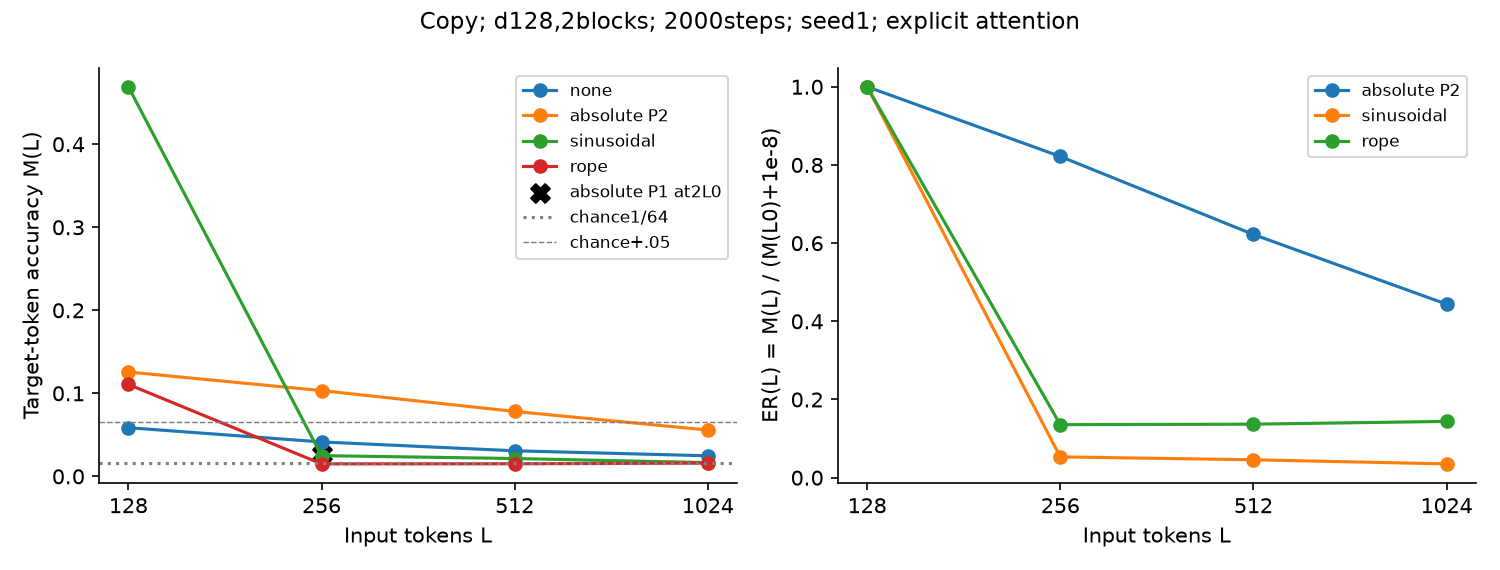
\includegraphics[width=\linewidth,height=.42\textheight,keepaspectratio]{figures/curves.png}
\caption{E1: точность и ER на новых длинах без дообучения; absolute использует P2.}\label{fig:curves}
\end{figure}

Синусоида лучше при обучающей длине, но уже на 256 её точность снижается до 0.024963. P2 даёт меньшую точность на $L_0$, зато сохраняет преимущество на длинных входах. Для none ER не интерпретируется как перенос навыка: уже исходный результат близок к частотному уровню и ниже практического порога. Все длины поместились в память.

Первая измеренная длина больше $L_0$ с $M\le0.065625$: P2 --- 1024, синусоида и RoPE --- 256. У none условие выполнено уже на 128, а первая более длинная точка --- 256. Максимальные проверенные длины выше порога: P2 --- 512, синусоида и RoPE --- 128. Это границы сетки для данного генератора, а не универсальная длина контекста.
\begin{figure}[H]\centering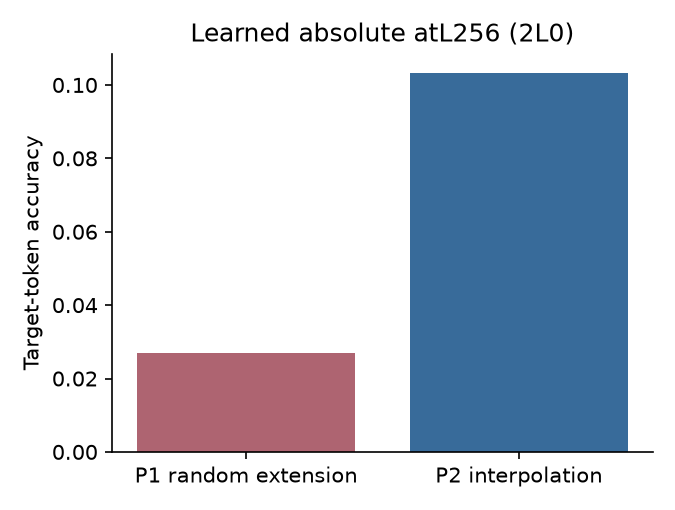
\includegraphics[width=\linewidth,height=.27\textheight,keepaspectratio]{figures/p1p2.png}
\caption{Сравнение P1 и P2 при удвоении длины для одних обученных весов.}\label{fig:p1p2}
\end{figure}

\begin{figure}[H]\centering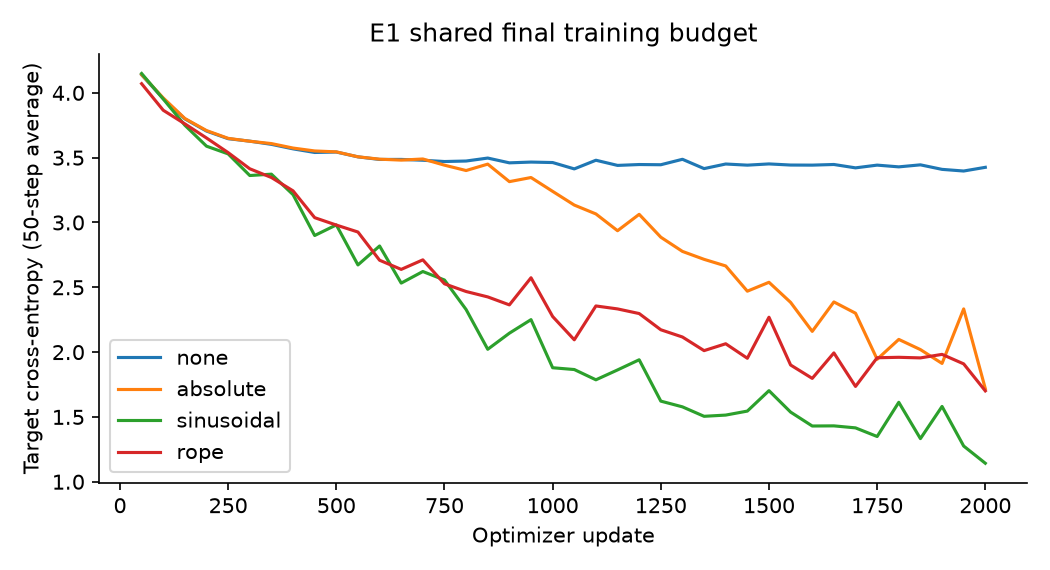
\includegraphics[width=\linewidth,height=.37\textheight,keepaspectratio]{figures/loss.png}
\caption{Train loss четырёх режимов позиции при общем бюджете 2000 обновлений.}\label{fig:loss}
\end{figure}

\section{E2. Измеренная стоимость внимания}
Профилирование не является обучающим сравнением: случайные веса фиксированы, batch 4, FP16. Каждая точка измерена в отдельном процессе после 10 прогревов по 30 повторам с синхронизацией CUDA; пик --- фактический максимум распределителя. Сравниваются explicit и принудительно выбранный efficient SDPA. FlashAttention в этой сборке Windows недоступен, поэтому efficient не обозначается как Flash.
\begin{table}[H]\centering\footnotesize
\setlength{\tabcolsep}{4pt}
\caption{E2: средние времена после прогрева и измеренный пик CUDA, batch 4, FP16.}\label{tab:e2}
\begin{tabular}{llrrrrl}
\toprule
Backend & $L$ & Forward, мс & Шаг, мс & Пик, MiB & Токен/с & Ист. \\
\midrule
explicit & 64 & 2.252 & 8.739 & 68.549 & 113659 & R17 \\
explicit & 128 & 2.461 & 9.264 & 71.023 & 208019 & R18 \\
explicit & 256 & 2.283 & 9.670 & 80.345 & 448472 & R19 \\
explicit & 512 & 3.198 & 9.318 & 114.884 & 640374 & R20 \\
explicit & 1024 & 2.975 & 9.176 & 243.962 & 1376727 & R21 \\
efficient & 64 & 1.840 & 8.365 & 68.307 & 139102 & R22 \\
efficient & 128 & 1.757 & 7.599 & 69.984 & 291369 & R23 \\
efficient & 256 & 1.798 & 7.929 & 73.852 & 569427 & R24 \\
efficient & 512 & 1.686 & 7.405 & 81.930 & 1214745 & R25 \\
efficient & 1024 & 2.835 & 9.243 & 98.086 & 1445015 & R26 \\
\bottomrule
\end{tabular}
\end{table}


\begin{table}[H]\centering\small
\setlength{\tabcolsep}{4pt}
\caption{Наклоны log--log регрессии по пяти длинам и по двум наибольшим.}\label{tab:slopes}
\begin{tabular}{llrr}
\toprule
Backend & Величина & $\alpha_{all}$ & $\alpha_{512,1024}$ \\
\midrule
explicit & Время forward & 0.118089 & -0.104255 \\
explicit & Время шага & 0.014908 & -0.022257 \\
explicit & Пик памяти & 0.435671 & 1.086481 \\
efficient & Время forward & 0.118652 & 0.749570 \\
efficient & Время шага & 0.025052 & 0.319792 \\
efficient & Пик памяти & 0.127139 & 0.259660 \\
\bottomrule
\end{tabular}
\end{table}


\begin{figure}[H]\centering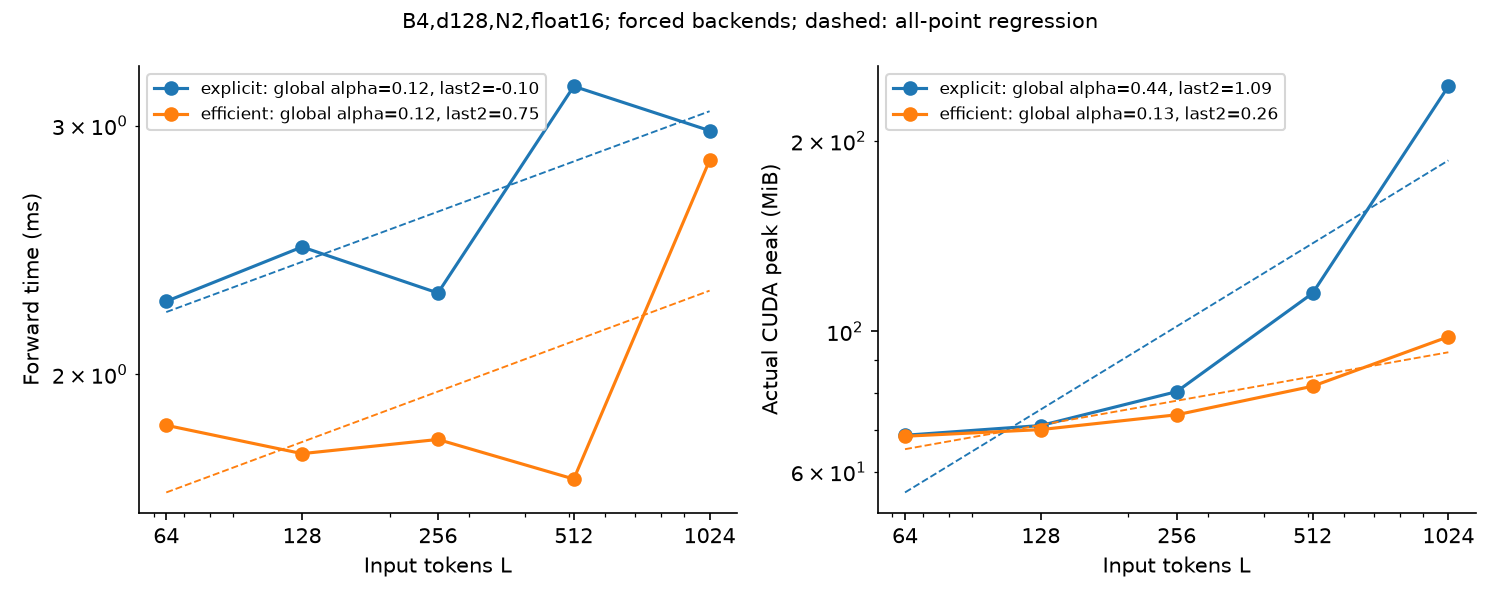
\includegraphics[width=\linewidth,height=.42\textheight,keepaspectratio]{figures/cost.png}
\caption{E2: измеренная стоимость explicit и efficient SDPA; log--log регрессии.}\label{fig:cost}
\end{figure}

Теоретическая стоимость блока имеет слагаемые $L^2d$ и $Ld^2$. В данной архитектуре MAC произведений внимания равен $2BL^2d$, проекций и FFN --- $8BLd^2$; отношение равно $L/(4d)$ и меняется от 0.125 до 2. Полный пик памяти включает веса, состояния оптимизатора, линейные активации и временные буферы.

Глобальные наклоны памяти 0.435671 и 0.127139 не попали в интервалы 1.6--2.4 для явного и 0.8--1.2 для эффективного внимания. Этот отрицательный результат сохраняется. Время немонотонно и не подтверждает квадратичный асимптотический режим. По допускаемому в разделе 9.2 задания способу выполнено неотрицательное описательное разложение $aL^2+bL+c$. На $L=1024$ доли этих компонент в пике: explicit 66.72\%, 5.90\%, 27.38\%; efficient 1.43\%, 31.03\%, 67.55\%. Фиксированная составляющая уменьшает наблюдаемый наклон. Пять длин не позволяют причинно отождествить каждый коэффициент с отдельным механизмом. Подстановка теоретического размера $A$ вместо измеренного пика здесь не используется.

\section{Диагностика внимания}
Для лучшей по val синусоидальной модели сохранены 256 последовательностей на каждой длине. По каждой голове отдельно рассчитаны
\begin{equation}H_i=-\sum_j A_{ij}\ln(A_{ij}+\varepsilon),\quad D_i=\sum_jA_{ij}|i-j|,\quad \mu_i(16)=\sum_{|i-j|\le16}A_{ij}.\end{equation}
Также показаны максимальный вес строки, масса на соответствующем исходном символе $\mu_{tgt}$ и энтропия на позициях ответа $H_{ans}$. Остальные средние берутся по всем query и объектам, масса цели --- по целевым позициям.
\begin{table}[H]\centering\footnotesize
\setlength{\tabcolsep}{4pt}
\caption{Диагностика синусоидальной модели по головам: R27 при $L=128$ и R28 при $L=256$.}\label{tab:attention}
\begin{tabular}{rrrrrrrrr}
\toprule
$L$ & Блок & Гол. & $H$ & $D$ & $\mu(16)$ & $\max A$ & $\mu_{tgt}$ & $H_{ans}$ \\
\midrule
128 & 1 & 1 & 4.0864 & 50.6866 & 0.1602 & 0.0611 & 0.0115 & 4.6631 \\
128 & 1 & 2 & 3.8492 & 55.4976 & 0.0885 & 0.0728 & 0.0146 & 4.1606 \\
128 & 1 & 3 & 4.2182 & 53.4020 & 0.1149 & 0.0421 & 0.0209 & 4.4416 \\
128 & 1 & 4 & 4.3923 & 40.9418 & 0.2781 & 0.0406 & 0.0081 & 4.4746 \\
128 & 2 & 1 & 2.0715 & 45.1388 & 0.2309 & 0.2988 & 0.2231 & 1.7876 \\
128 & 2 & 2 & 2.0912 & 45.5602 & 0.2321 & 0.2908 & 0.2202 & 1.8238 \\
128 & 2 & 3 & 2.1303 & 45.4354 & 0.2299 & 0.2817 & 0.2201 & 1.8415 \\
128 & 2 & 4 & 2.1185 & 44.9189 & 0.2416 & 0.2802 & 0.2262 & 1.8339 \\
256 & 1 & 1 & 5.0163 & 96.1305 & 0.0674 & 0.0194 & 0.0049 & 5.3194 \\
256 & 1 & 2 & 4.3674 & 112.0862 & 0.0218 & 0.0481 & 0.0089 & 4.0874 \\
256 & 1 & 3 & 4.9851 & 107.1343 & 0.0434 & 0.0223 & 0.0081 & 4.8035 \\
256 & 1 & 4 & 4.9017 & 106.9133 & 0.0583 & 0.0245 & 0.0087 & 4.8682 \\
256 & 2 & 1 & 2.9694 & 100.2339 & 0.1205 & 0.2039 & 0.0085 & 2.4816 \\
256 & 2 & 2 & 2.8748 & 101.9694 & 0.1154 & 0.2128 & 0.0078 & 2.3935 \\
256 & 2 & 3 & 2.9838 & 103.6340 & 0.1215 & 0.1925 & 0.0083 & 2.5291 \\
256 & 2 & 4 & 3.0121 & 102.5506 & 0.1242 & 0.1798 & 0.0082 & 2.5281 \\
\bottomrule
\end{tabular}
\end{table}


\begin{figure}[H]\centering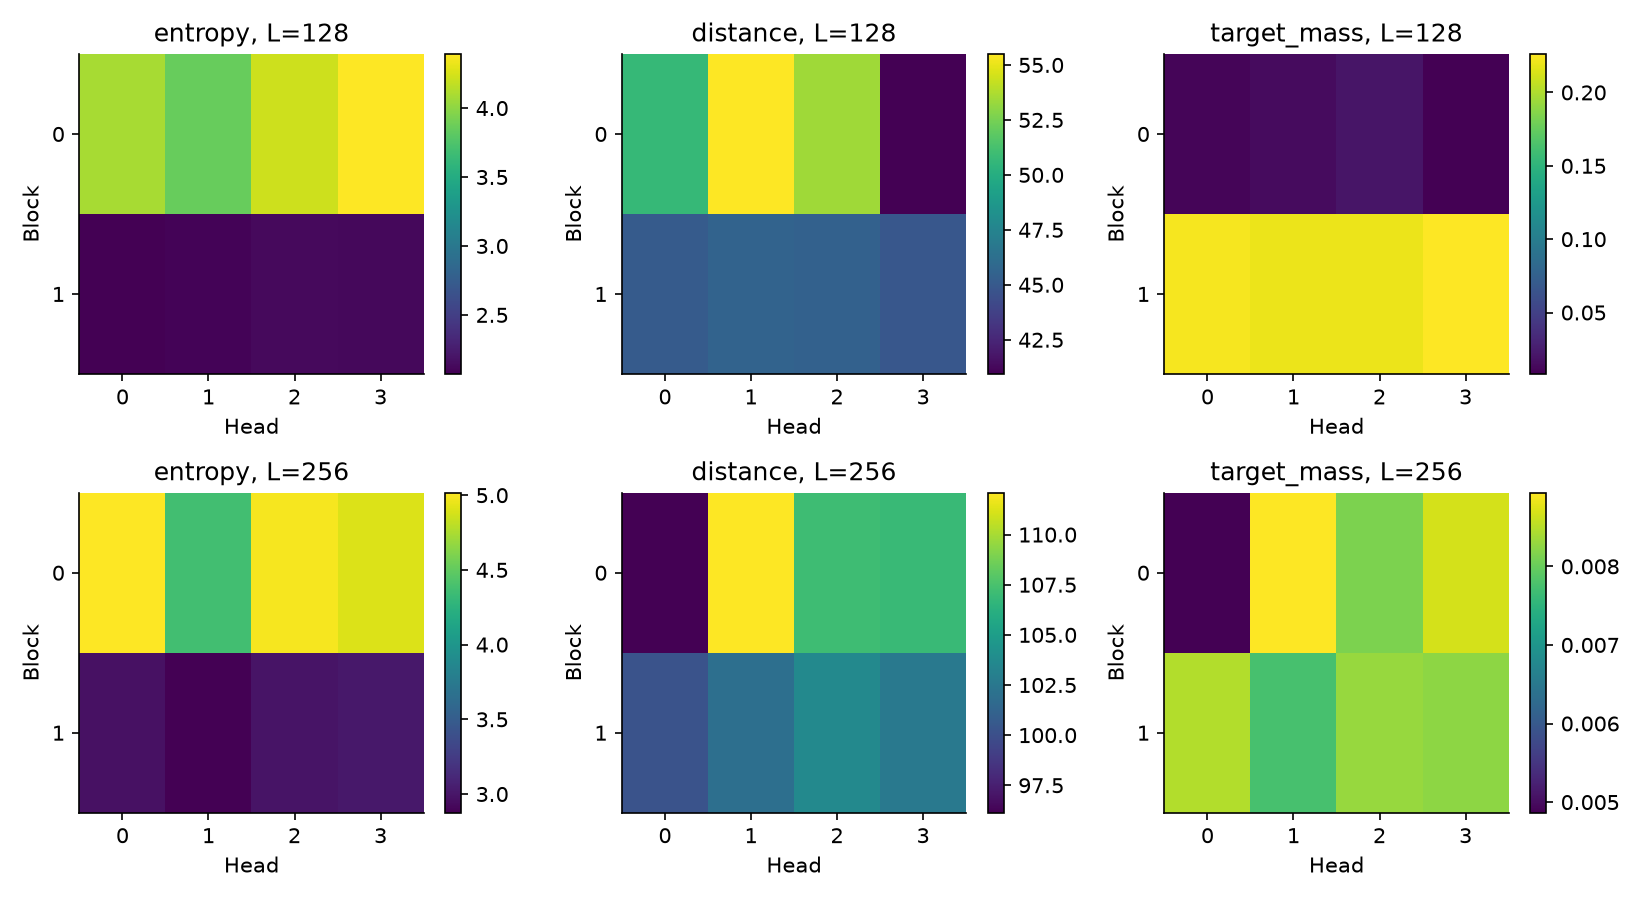
\includegraphics[width=\linewidth,height=.43\textheight,keepaspectratio]{figures/heads.png}
\caption{Энтропия, расстояние и масса внимания по головам синусоидальной модели.}\label{fig:heads}
\end{figure}

Во втором блоке средняя масса на нужном исходном символе падает с 0.222375 до 0.008194, одновременно с падением точности. Среднее расстояние растёт примерно с 45 до 102 токенов, масса в окне 16 уменьшается. Энтропия тоже зависит от длины, поэтому её сравнение учитывает изменение числа ключей: равномерная строка имеет $\ln L$. Эти наблюдения согласуются с нарушением маршрутизации, но карта внимания не доказывает необходимость конкретной головы без вмешательства.

\section{E3. Основное сравнение на трёх seed}
До дополнительных запусков зафиксирована гипотеза $M_{RoPE}(256)-M_{P2}(256)<0$: интерполяция P2 может лучше сохранить используемую сетку, тогда как относительная форма RoPE сама по себе не обеспечивает переноса. Единственный изменяемый фактор --- позиционное представление. Архитектура, LR, бюджет, генератор, explicit backend и длина оценки фиксированы. Нулевая либо положительная разность или отсутствие устойчивости по критерию задания опровергли бы ожидаемый установленный отрицательный эффект. Seed 1 повторно использует веса E1; seed 2 и 3 независимы и общие для пары.
\begin{table}[H]\centering\small
\setlength{\tabcolsep}{4pt}
\caption{E3: RoPE минус абсолютная таблица P2, $L^*=256$.}\label{tab:e3}
\begin{tabular}{lrrrl}
\toprule
Seed & RoPE & P2 & $\Delta_s$ & Источники \\
\midrule
1 & 0.015015 & 0.103271 & -0.088257 & R29/R30 \\
2 & 0.022491 & 0.093964 & -0.071472 & R31/R32 \\
3 & 0.017029 & 0.073639 & -0.056610 & R33/R34 \\
\bottomrule
\end{tabular}
\end{table}


\begin{figure}[H]\centering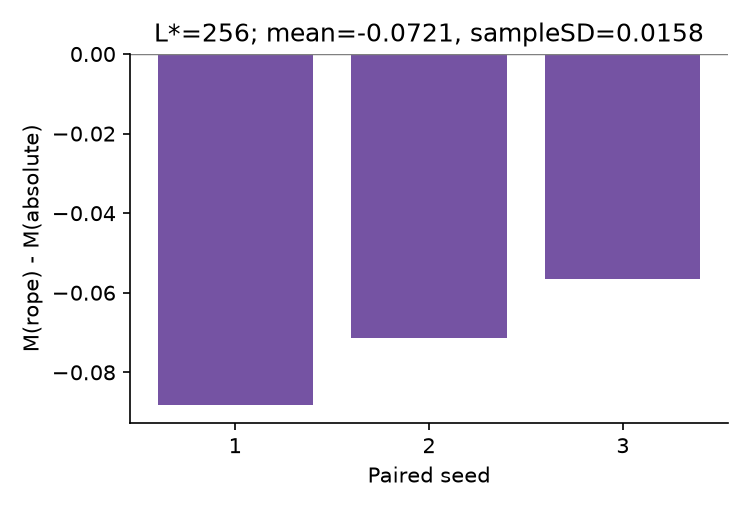
\includegraphics[width=\linewidth,height=.29\textheight,keepaspectratio]{figures/paired.png}
\caption{Три парные разности RoPE минус P2.}\label{fig:paired}
\end{figure}

Средняя разность равна $-0.072113$, выборочное SD --- 0.015833. Все три значения отрицательны и $|\overline\Delta|\ge2s_\Delta=0.031666$: различие установлено в пользу P2, гипотеза поддержана. Вывод относится к copy, длине 256 и данному рецепту; он не переносится автоматически на естественные тексты.

\section{Ответы на контрфактические вопросы}
\subsection*{Вопрос 1. Определённость синусоиды и перенос}
На максимальной длине 1024 синусоида даёт $M=0.016548$, $ER=0.035271$ (R12). Модель обучалась только до 128. Новые фазы и расстояния формально допустимы, однако закономерность копирования на них не была освоена. Определённость вектора позиции не является гарантией качества.
\subsection*{Вопрос 2. Четырёхкратное увеличение длины}
При 256 $\to$ 1024 число элементов $A$ растёт в $4^2=16$ раз. Фактический пик explicit растёт в 3.036440 раза, efficient --- в 1.328150 (R19/R21 и R24/R26). Парные наклоны равны $\log(3.036440)/\log4=0.801190$ и 0.204709. Фиксированные и линейные компоненты пика объясняют отличие от чистого размера матрицы; efficient не хранит полную матрицу $A$.
\subsection*{Вопрос 3. P1 против P2}
При 256 получены $M_{P1}=0.027008$ (R35) и $M_{P2}=0.103271$ (R06). Разность P2 минус P1 равна 0.076263. P1 добавляет случайные необученные строки, P2 интерполирует всю сетку внутри обученного диапазона и меняет расстояния между кодами. Числа характеризуют два правила для одних весов без дообучения.
\subsection*{Вопрос 4. Одна длина и вся кривая}
Даже преимущество RoPE на одной длине не означало бы независимость навыка от длины. В собственных данных RoPE уступил P2 на всех четырёх длинах, а три разности E3 отрицательны. Его $M$ изменяется с 0.110718 до 0.015938, то есть навык явно не сохраняется. Установленный знак E3 относится только к выбранной длине и генератору.
\subsection*{Вопрос 5. Удвоение ширины}
При $L=512$, $d:128\to256$ сохранённые времена forward равны 2.299830 и 3.128763 мс (R36 / R37), отношение 1.360432. Члены $L^2d$ и $Ld^2$ увеличиваются в 2 и 4 раза. При исходных размерах их MAC-вклады равны, поэтому суммарный теоретический рост --- в 3 раза. Замер ближе к 2, но ниже обоих чистых множителей: фиксированные расходы и загрузка GPU существенны, а близость к 2 не доказывает доминирования одного члена.

\noindent\textbf{Заключение.} Максимальная длина, помещающаяся в память, не совпала с длиной сохранения навыка. P2 оказался устойчивее RoPE на выбранном режиме, хотя синусоида лучше на обучающей длине. Полный пик и время на данной сетке не достигли простых асимптотических режимов; разложение стоимости позволяет описать это ограничение без подмены измерений.
\clearpage
\renewcommand{\refname}{Список использованных источников}
\begin{thebibliography}{9}
\addcontentsline{toc}{section}{Список использованных источников}
\bibitem{teacher} Лабораторная работа 3. Attention и моделирование длинных последовательностей. Positional representations, extrapolation, complexity и local attention. Курс «Нейронные сети». Методические указания, 2026.
\end{thebibliography}
\clearpage
\section*{Приложение. Идентификация запусков}
\addcontentsline{toc}{section}{Приложение. Идентификация запусков}
\begingroup\small\setstretch{1.05}
\begin{longtable}{@{}l>{\raggedright\arraybackslash}p{3.5cm}p{10.8cm}@{}}
\caption{Полные RUN\_ID источников результатов.}\\
\toprule Код & Условие & RUN\_ID \\ \midrule \endhead
\hypertarget{R01}{R01} & E1 none L128 & {\fontsize{8.8}{11}\selectfont\texttt{39a1e67c568afe0e37ae-fbdaf429f02949d3aa954ef0a7413191}} \\
\hypertarget{R02}{R02} & E1 none L256 & {\fontsize{8.8}{11}\selectfont\texttt{f114fe509648da7b49f7-1b8c6edd068e418bac214fba181fdd09}} \\
\hypertarget{R03}{R03} & E1 none L512 & {\fontsize{8.8}{11}\selectfont\texttt{e1ac564e288280b848d4-502bea42f55047859fa3a1731b1f1bda}} \\
\hypertarget{R04}{R04} & E1 none L1024 & {\fontsize{8.8}{11}\selectfont\texttt{6de547c4c16e6eb48409-a3de018b67e940b582cf6a3f528614ae}} \\
\hypertarget{R05}{R05} & E1 absolute L128 & {\fontsize{8.8}{11}\selectfont\texttt{d736946de91b20c626c4-a6f215ba70b84066af2d941dbbe12ee7}} \\
\hypertarget{R06}{R06} & E1 absolute L256 & {\fontsize{8.8}{11}\selectfont\texttt{845d705bc5bb903516c8-748407084dd1465c887abe46f362f47d}} \\
\hypertarget{R07}{R07} & E1 absolute L512 & {\fontsize{8.8}{11}\selectfont\texttt{f8074c189505727e0ccf-3981eb86dc464a3f9f68f8031b5af2f2}} \\
\hypertarget{R08}{R08} & E1 absolute L1024 & {\fontsize{8.8}{11}\selectfont\texttt{cb812fc715c93835c683-84b994ebe1e346af8b5ed4bd654ca86a}} \\
\hypertarget{R09}{R09} & E1 sinusoidal L128 & {\fontsize{8.8}{11}\selectfont\texttt{ba603459beba7c94148e-5e3c9760ad2e49f9872957427a668afd}} \\
\hypertarget{R10}{R10} & E1 sinusoidal L256 & {\fontsize{8.8}{11}\selectfont\texttt{8c10d0590ae01638d9dd-7337e208cccc48fda1929186f0f36f01}} \\
\hypertarget{R11}{R11} & E1 sinusoidal L512 & {\fontsize{8.8}{11}\selectfont\texttt{4d707f93887c3d8b4457-251ba15323f044d7a744e6bc931b3b9b}} \\
\hypertarget{R12}{R12} & E1 sinusoidal L1024 & {\fontsize{8.8}{11}\selectfont\texttt{a52079b305a573b0a345-873c9a3089794dd7adb24c832d642ab5}} \\
\hypertarget{R13}{R13} & E1 rope L128 & {\fontsize{8.8}{11}\selectfont\texttt{61fdba3d7d201fa4d57f-a4b611115fa4462a806c8e87183cadcf}} \\
\hypertarget{R14}{R14} & E1 rope L256 & {\fontsize{8.8}{11}\selectfont\texttt{3b50ed6e7f33d6181d3f-f56b595426f14655b5f51ccd12feda63}} \\
\hypertarget{R15}{R15} & E1 rope L512 & {\fontsize{8.8}{11}\selectfont\texttt{2d84c8b5e95f6e3f3142-7b9aff603250409484ac8d6dfaa1ce25}} \\
\hypertarget{R16}{R16} & E1 rope L1024 & {\fontsize{8.8}{11}\selectfont\texttt{92370f1efe2928f08dd0-7aab1815493d4fb482d0e0beb0ec0f06}} \\
\hypertarget{R17}{R17} & E2 explicit L64 & {\fontsize{8.8}{11}\selectfont\texttt{24f7a8ba7960c3f9e999-f228a00ba2c347bcbb206618a346bcf5}} \\
\hypertarget{R18}{R18} & E2 explicit L128 & {\fontsize{8.8}{11}\selectfont\texttt{a7b35549eff6ece9eb69-a9b4449f96a24e4292114bc491bdc52d}} \\
\hypertarget{R19}{R19} & E2 explicit L256 & {\fontsize{8.8}{11}\selectfont\texttt{e5d04a9497324471d3a0-e6e5c7472e18460ea27e19556d23e10b}} \\
\hypertarget{R20}{R20} & E2 explicit L512 & {\fontsize{8.8}{11}\selectfont\texttt{4931af932992351dfa50-cec56a3b47ad417a8c33b962b88da271}} \\
\hypertarget{R21}{R21} & E2 explicit L1024 & {\fontsize{8.8}{11}\selectfont\texttt{a086c993bc6d504fa01c-c14c5e9c287546348a7e18640a62bf27}} \\
\hypertarget{R22}{R22} & E2 efficient L64 & {\fontsize{8.8}{11}\selectfont\texttt{1550b6a9b24f1e551915-4edd8677db9c4fe19e100650ebfae848}} \\
\hypertarget{R23}{R23} & E2 efficient L128 & {\fontsize{8.8}{11}\selectfont\texttt{6b665e12a6c53dfe2711-6bacc96b732a4dec945d276cfc54cb22}} \\
\hypertarget{R24}{R24} & E2 efficient L256 & {\fontsize{8.8}{11}\selectfont\texttt{54002e33bd89266b4aa0-5d661f49f1044fb7ac129f098f820b8b}} \\
\hypertarget{R25}{R25} & E2 efficient L512 & {\fontsize{8.8}{11}\selectfont\texttt{d07391af265a5628039e-173659cdb29b4766b24ffe9bd80cf1b3}} \\
\hypertarget{R26}{R26} & E2 efficient L1024 & {\fontsize{8.8}{11}\selectfont\texttt{e648147c7ab327beb2f0-876b5110f59748429fd2dd3d6c803968}} \\
\hypertarget{R27}{R27} & Attention L128 & {\fontsize{8.8}{11}\selectfont\texttt{57972cf22da5f30ef01e-53864dfbbfa643008504498d71bbd92b}} \\
\hypertarget{R28}{R28} & Attention L256 & {\fontsize{8.8}{11}\selectfont\texttt{982d0e8b62adcf1060bb-8e10b294ace440fc9b6ed4ad48b6481c}} \\
\hypertarget{R29}{R29} & E3 rope s1 & {\fontsize{8.8}{11}\selectfont\texttt{73af15a95254a9e7505e-2e6fac200dc94a5cb29771d88a799892}} \\
\hypertarget{R30}{R30} & E3 absolute s1 & {\fontsize{8.8}{11}\selectfont\texttt{81e535c7a7b9c0de7464-43393f737a44426d8e19b60afe00a413}} \\
\hypertarget{R31}{R31} & E3 rope s2 & {\fontsize{8.8}{11}\selectfont\texttt{193c197aef769453e75d-e9a9467ad1ae40259380dc6fa5f2de8a}} \\
\hypertarget{R32}{R32} & E3 absolute s2 & {\fontsize{8.8}{11}\selectfont\texttt{f8268a85bca09e3e6428-fb23fd829ffb493996177de32bea4628}} \\
\hypertarget{R33}{R33} & E3 rope s3 & {\fontsize{8.8}{11}\selectfont\texttt{eb89d1360a5bbf004cd5-db43c23a876243ef9b928d34e4eeb852}} \\
\hypertarget{R34}{R34} & E3 absolute s3 & {\fontsize{8.8}{11}\selectfont\texttt{91d130aa0b251a01039b-c16e40fd77ae43b48536503b6812c710}} \\
\hypertarget{R35}{R35} & P1 L256 & {\fontsize{8.8}{11}\selectfont\texttt{6b6c3022238da3f20ce2-57fd7d84b9754079827c89cfc1f1bcef}} \\
\hypertarget{R36}{R36} & CF5 width 128 & {\fontsize{8.8}{11}\selectfont\texttt{2441610fedefbc0a2067-a9deed5346cb43c9b4fb0663612cd0ac}} \\
\hypertarget{R37}{R37} & CF5 width 256 & {\fontsize{8.8}{11}\selectfont\texttt{f4afe447f7b29d71c175-487015fc65f842b19e08b2a8a161bd32}} \\
\bottomrule\end{longtable}\endgroup
